\title{Box2D Group 21 Project Report}
\author
{
  \texttt{130070009}
  Anand Dhoot\\
  \and
  \texttt{13D100004}
  Maulik Shah\\
  \and
  \texttt{13D100032}
  Anchit Gupta\\
}
\maketitle

\newif\iflattersubsect
\lattersubsecttrue

\AtBeginSection[]
{
	\iflattersubsect
   \begin{frame}
       \frametitle{Overview}
       \tableofcontents[sections]
   \end{frame}
   \fi
   \lattersubsectfalse
}

\section{Introduction}
\begin{frame}
\frametitle{Introduction}
A Rube-Goldberg machine is a deliberately over-engineered or overdone machine that performs a very simple task in a very complex fashion, usually including a chain reaction. We have designed once such contraption using Box2D, which we present here. 
\pause
\\
\\
Inspired by the festive season and our love for fireworks we decided to go with a festive theme. A very clever boy loves fireworks but is
afraid to light them and just likes to see them from a distance. After starting this Rube Goldberg machine and positioning the fireworks the boy gets enough time to go back a safe distance and climb on to the roof of his house to witness the show. 
\end{frame}

\section{Schematic}
\begin{frame}
\frametitle{Original Schematic}
\begin{center}
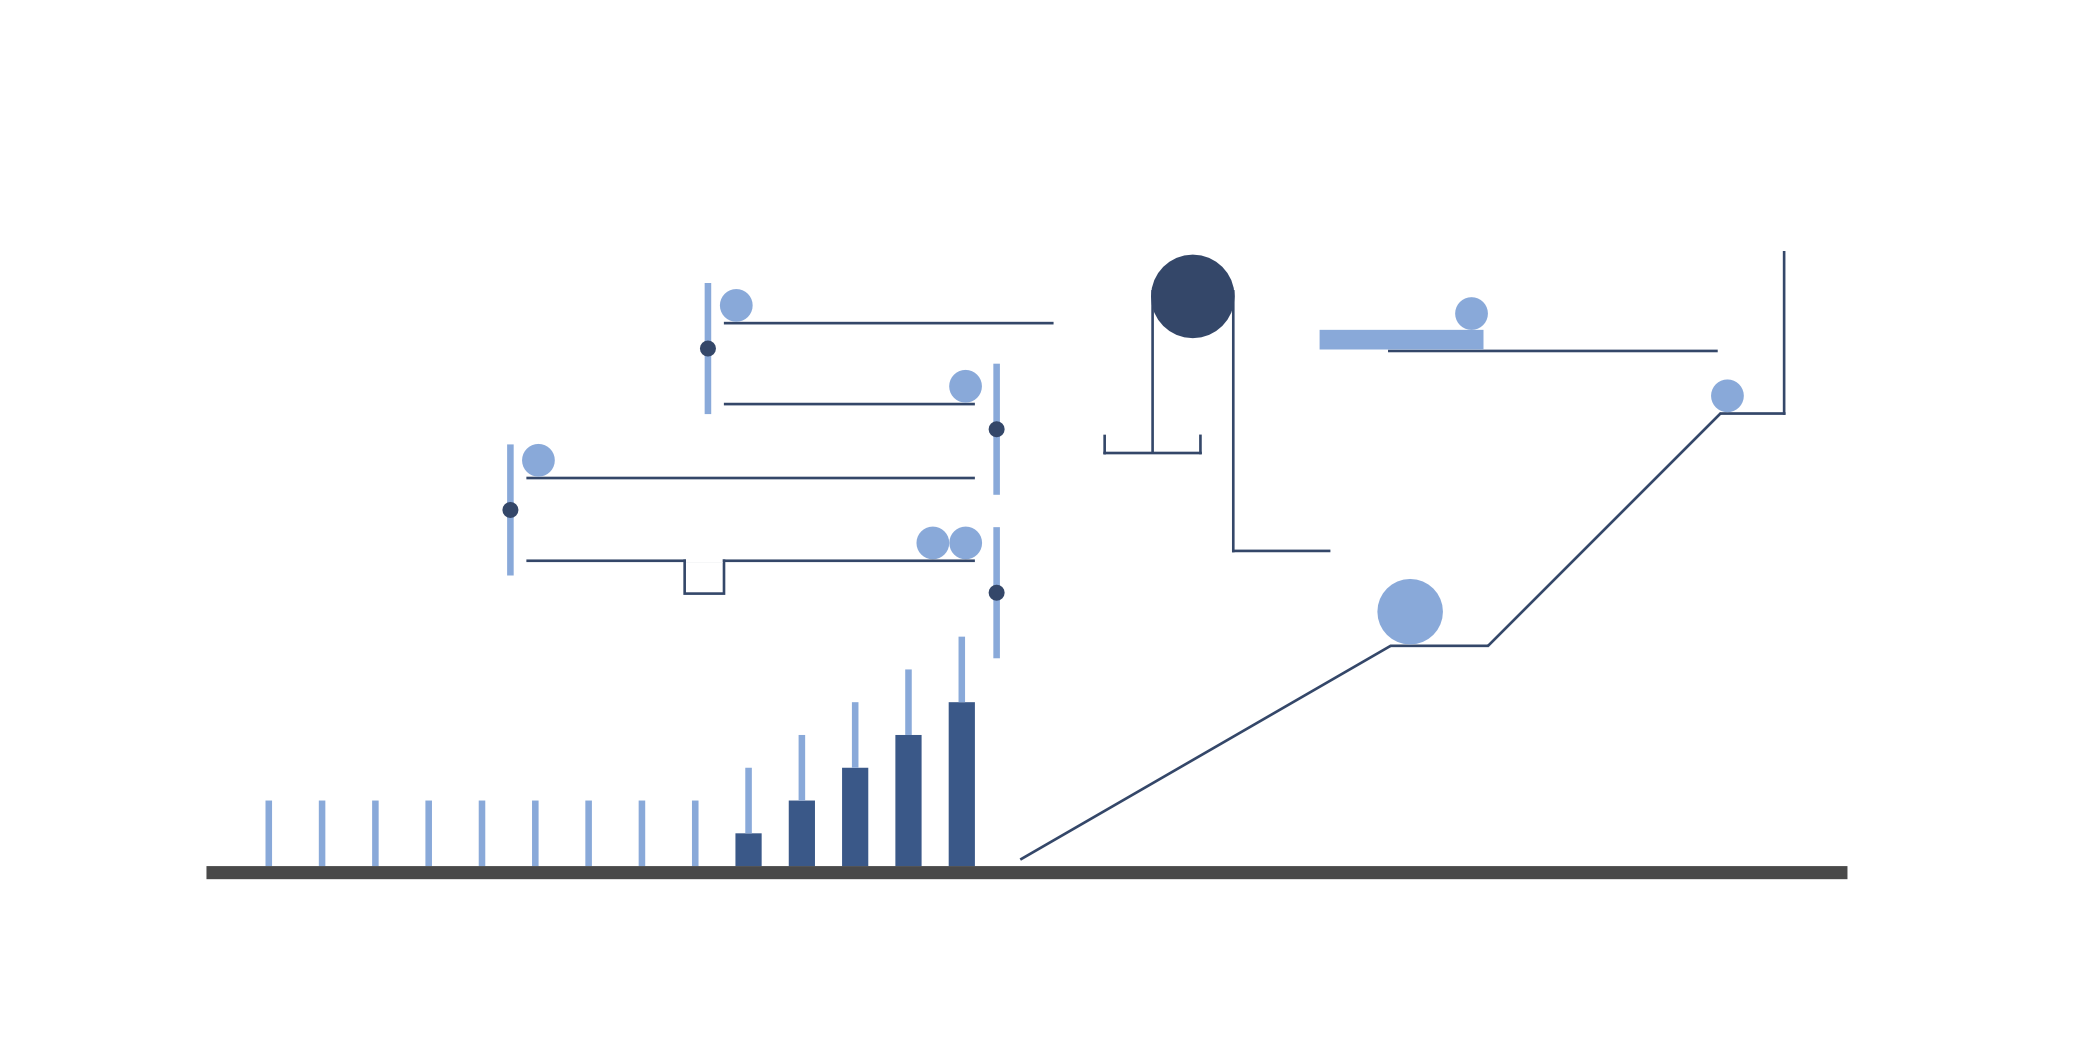
\includegraphics[scale=1.1]{./Images/rect3049.png}
\end{center}
\end{frame}

\begin{frame}
\frametitle{Final Design}
\begin{center}
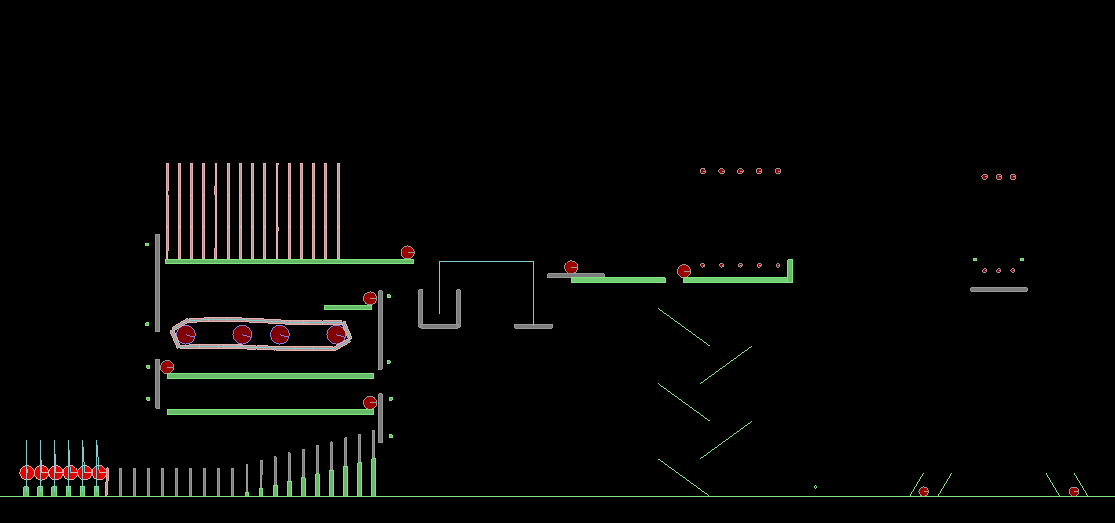
\includegraphics[scale=0.27]{./Images/FinalDesign.png}
\end{center}
\end{frame}

\section{Components Used}
\begin{frame}
	\frametitle{Components Used}
\begin{itemize}
\item Newton's Pendulum
\item Dominos
\item Conveyor Belt
\item Pulleys
\item Explosions
\item Cannons
\end{itemize}
\end{frame}

\subsection{Newton's Pendulum}
\begin{frame}
  \frametitle{Newton's Pendulum}
  \begin{center}
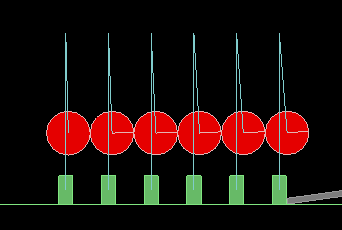
\includegraphics[scale=.45]{./Images/NewtonsPendulum.png}
  \end{center}
Newton's Pendulum is basically a set of adjacent simple pendulums which  beautifully demonstrates the principles of momentum conservation, energy conservation and impulses.
\end{frame}


\subsection{Dominos}
\begin{frame}
\frametitle{Dominos}
\begin{center}
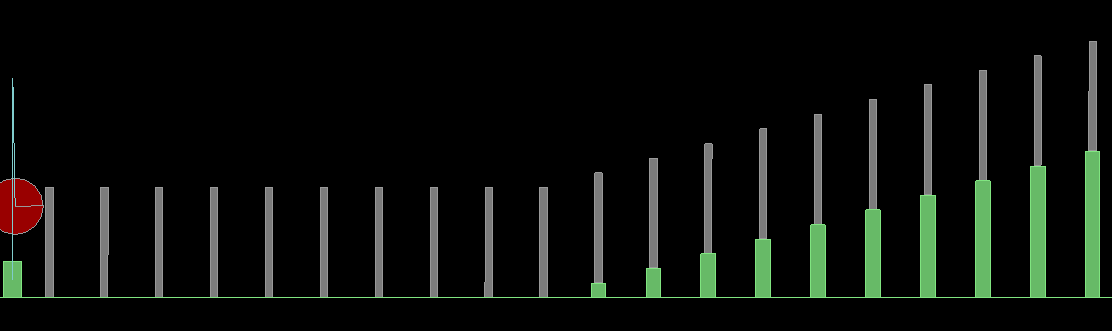
\includegraphics[scale=.25]{./Images/LowerDominos.png}
\end{center}
Dominos are a series of thin planks placed closed to each other. They give rise to a chain reaction when the first domino topples as each domino, on toppling, in turn topples the next domino and so on. This a great exapmlpe of impulse transfer resulting in a chain reaction.
\\
\pause
Dominoes have been used quite a bit in the simulation as means to quickly tranfer momentum to the subsequent parts of the machine.
\end{frame} 

\subsection{Conveyor Belt}
\begin{frame}
\frametitle{Conveyor Belt}{Conveyor Belt}
\begin{center}
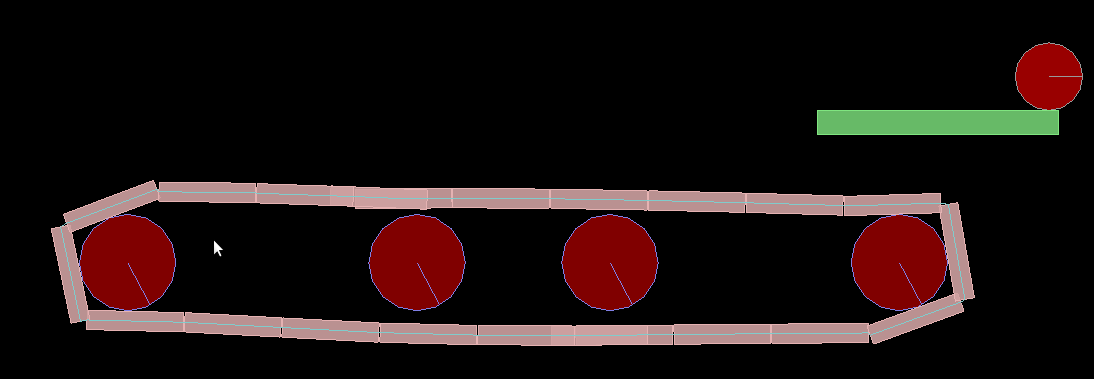
\includegraphics[scale=.25]{./Images/ConveyorBelt.png}
\end{center}
The conveyor belt has the ability to mechanise bodies. The conveyor belt in our design carries the ball from one side to another quickly. 
\\
\pause
The idea was implemented as a rectangular chain with rotating high friction discs between the chain. we give the discs a constant angular velocity, due to which the conveyor belt rotates.
\end{frame}

\subsection{Pulleys}
\begin{frame}
  \frametitle{Pulleys}
  \begin{center}
  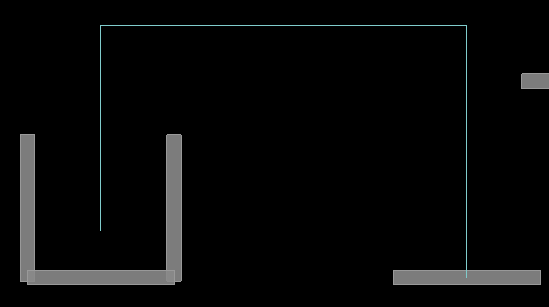
\includegraphics[scale=0.25]{./Images/Pulley.png}
  \end{center}
We have used to pulley as an element of the Rube Goldberg machine to trigger the next set of events. When the ball falls into one side of the pulley, which causes the right side to move up. Essentially, this uses the force of gravity on the ball to push the plank on the right upwards for the next stage of the simulation.
\end{frame}


\subsection{Explosions}
\begin{frame}
  \frametitle{Explosions}
  \begin{center}
  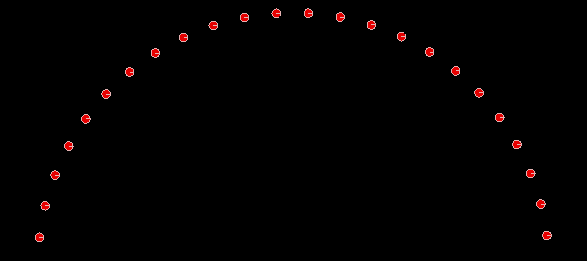
\includegraphics[scale = 0.25]{./Images/Explosion00.png}
  \end{center}
  This element is the centerpiece of our whole simulation. We have placed multiple triggers and fireworks all around the simulation
which are triggered at different times in the simulation. Going with the theme of the festive season these explosion we think quite 
realistically simulate the real deal and add a element of novelty and uniqueness to our project.
\end{frame} 


\subsection{Cannons}
\begin{frame}
  \frametitle{Cannons}
  \begin{center}
  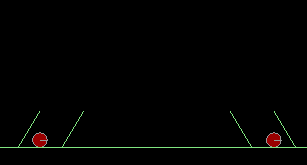
\includegraphics[scale=0.25]{./Images/Cannon00.png}
  \end{center}
The finale of our simulation is triggered by two canons which launch a projectile. Using this we have carefully alligned them so as that they converge to a common point $\oplus$ and thus be able to provide enough force so as to push the plank which triggers the finale.
\end{frame} 


\section{Challenging Aspects}
\subsection{Conveyor Belt}
\begin{frame}
\frametitle{Conveyor Belt}
The conveyor belt in Box2D can be implemented in many ways. \pause One of them include applying a force/impulse on any contacting body. \pause This seems quite non intuitive and wouldnt have resulted in a realistic simualtion. 
\\ 
\pause
So we decided to go the hard route and implement our own realistic Conveyor belt. This involved making the conveyor belts from links which which were then joined by revolute joints. The rotating force is supplied by the 4 rollers below the belt which have been given a angular velocity and high friction.
\end{frame}

\subsection{Explosions}
\begin{frame}{Explosions} 
One of the most exciting new elements that we added in our design post the midsemester evaluation is the use of triggered fireworks i.e explosions. 
\\ 
\pause
To achieve an appropriate triggering action we had to define our own contact solver function. This involved manipulating the pointers to bodies in the world and subsequently checking whether the colliding/contacting bodies are the triggers and then triggering the explosion.
\end{frame}

\subsection{Modular Code}
\begin{frame}{Modular Code}
During the entire coding process, we followed good coding practices to ensure that our code is
\begin{itemize}
\item Maintainable
\item (Re)usable
\item Efficient
\item Documented
\end{itemize}
This hugely incresed the simplicity of the code and made it modular so that any part of it can be reused in some other project just by changing a few size/position variables. Extensive testing was done to position each element precisely and ensure that no element/machine of the simulation fails.
\end{frame}

\section{Conclusions}
\begin{frame}
	\frametitle{Conclusions}
We have discussed the various components of our Rube Goldberg machine; covering design, special features, and physical aspects behind components of our Rube Goldberg Machine.
\end{frame}

\section{References}
\begin{frame}
	\frametitle{References}
	\bibliographystyle{plain}
	\bibliography{ref}{}
	\cite{wiki:001} 
	\cite{wiki:002} 
	\cite{wiki:000} 
	\cite{website:coll}
	\cite{website:bod}
	\cite{website:fix}
	\cite{website:user}
	\cite{wiki:000} 
  \cite{website:you}
	\cite{website:git}
\end{frame}
